\documentclass{beamer}

    % INFO
    \title[Dance]{Everybody Dance Now}
    \author{Paul Comeau}
    \institute[CSM]{Colorado School of Mines}
    \date{9/14/2018}

    % Add your macros
    \input{macros}

    % PACKAGES
    \usepackage{montserrat}
    \usepackage{fontspec} 
    \usepackage{graphicx}
    \usepackage{setspace}
    \usepackage{tikz}
    % \usepackage{customtitleslide}
    \usepackage{booktabs} % book-quality tables
    \usepackage[ruled,vlined]{algorithm2e}

    % FUNCTIONS
    \AtBeginSection[]
    {
        \begin{frame}<beamer>
        \tableofcontents[currentsection]
        \end{frame}
    }

    % \AtBeginSubsection[]
    % {
    %     \begin{frame}<beamer>
    %     \tableofcontents[currentsubsection]
    %     \end{frame}
    % }

    % THEMING
    \usetheme{Madrid}
    \usecolortheme{mines}

\begin{document}

    %  Regular Title Slide
    {
    \begin{frame}[plain]
        \titlepage
        \centering
            
\includegraphics[width=0.25\textwidth]{images/logo.png}
    \end{frame}
    }

    \begin{frame}
        \frametitle{Overview}
        \begin{columns}
            \begin{column}{0.5\textwidth}
                \vspace{0.2in}
                This paper is an attempt to create a learning based pipeline for human motion. \\
                \vspace{0.2in}
                The algorithms are based on previous work in video rewrite technology, and motion matching between similar individuals and poses. Methods based on pix2pixHD objective. \\
                
            \end{column}
            \begin{column}{0.5\textwidth}
	     Let's take a look...
                \vspace{0.2in}
                
                \begin{center}
                \end{center}
            \end{column}
        \end{columns}
    \end{frame}

     \begin{frame}
        \frametitle{GANs}
               \begin{columns}
            \begin{column}{0.6\textwidth}
                \vspace{0.2in}
                Generative Adversarial Networks \\
                \vspace{0.2in}
                The end goal is to produce images which cannot be distinguished from the sample data set. Composed of two learning networks discriminator and a generator.\\
            \end{column}
            \begin{column}{0.4\textwidth}
                \vspace{0.2in}
                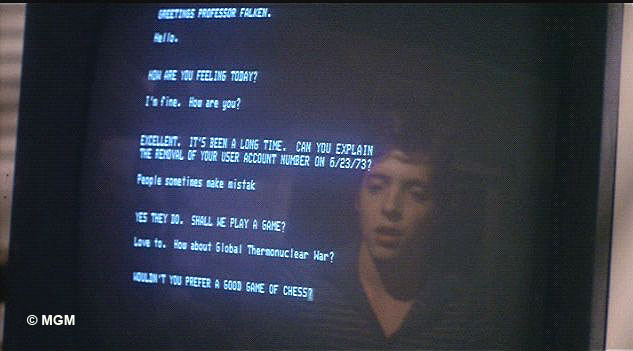
\includegraphics[scale=.3]{images/wargames-terminal.jpg}
                \begin{center}
                \end{center}
            \end{column}
        \end{columns}
    \end{frame}

     \begin{frame}
        \frametitle{GANs - Discriminator}
        A classifier that attempts to detect whether an image is generated (fake) or from the original data set. \\
        \vspace{0.2in}
        Given a succession of both real and generated images to train on.\\
        \vspace{0.2in}
        Gives a true or false result based on learned details that point towards an image being generated.
    \end{frame}

     \begin{frame}
        \frametitle{GANs - Generator}
        Produces images from random noise. \\
        \vspace{0.2in}
        Trained using gradient descent, based on discriminator error. This allows for more nuance in the adjustment of factors when producing an image, attempting to target factors which distinguish real and generated images.\\
    \end{frame}

    \begin{frame}
        \frametitle{GANs - Overview}
        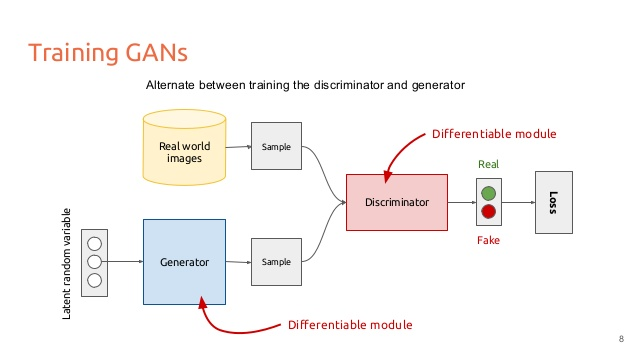
\includegraphics[scale=.5]{images/GANs.jpg}
    \end{frame}

    \begin{frame}
        \frametitle{Process Components}
        Pose Estimation and Mapping Training. \\
        \vspace{0.2in}
        Global Pose Normalization.\\
        \vspace{0.2in}
        Mapping From Source to Target
    \end{frame}

    \begin{frame}
        \frametitle{Pose Estimation}
        Goal - Encode body positions. \\
        \vspace{0.2in}
        Pose detector P accurately estimates the x,y joint positions in the target image.\\
        \vspace{0.2in}
        Stick figures are created from these coordinates, these figure images serve as inputs for mapping G. This process uses an adversarial discriminator D in order to differentiate between “real” and “fake” coordinate pairs. \\
        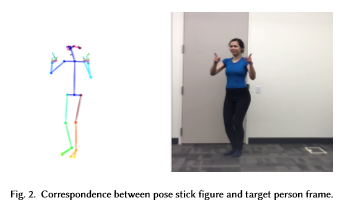
\includegraphics[scale=.8]{images/figure_example.png}
    \end{frame}

    \begin{frame}
        \frametitle{Pose Estimation Training}
        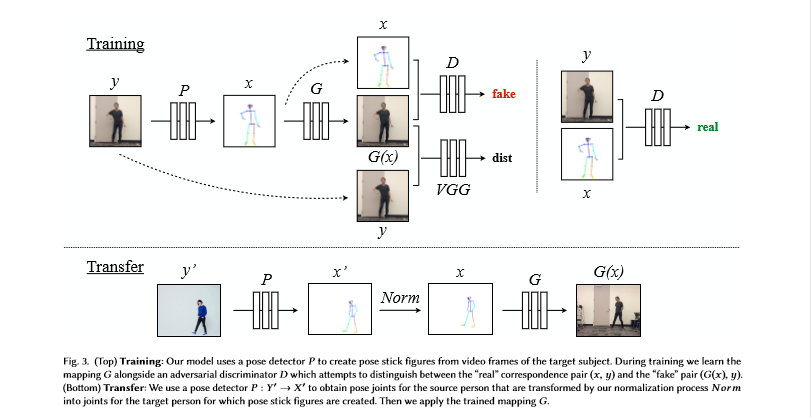
\includegraphics[scale=.6]{images/training.png}
    \end{frame}

    

    \begin{frame}
        \frametitle{Pose Normalization}
        To deal with different body proportions and distances from the camera, poses are normalized before they are applied to a target subject. \\
        \vspace{0.2in}
        Calculated by analyzing heights and ankle positions for both subjects and applying linear mapping between the furthest and closest ankle positions in both sample videos.\\
        \vspace{0.2in}
        These statistics used to calculate scale and translation for each frame between detected poses.
    \end{frame}

     \begin{frame}
        \frametitle{Translation}
        Detects pose from sample video (dancer or martial artist) with pose detector P. \\
        \vspace{0.2in}
        Normalizes pose using previously found global pose normalization. Applies learned mapping G to produce image of target individual performing originally detected pose.\\
        \vspace{0.2in}
        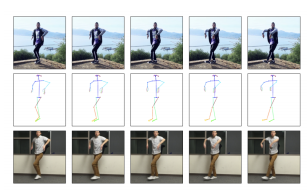
\includegraphics[scale=.8]{images/translate.png}
    \end{frame}

        \begin{frame}
        \frametitle{Pose Estimation Training - Smoothing Function}
            \begin{columns}
            \begin{column}{0.5\textwidth}
                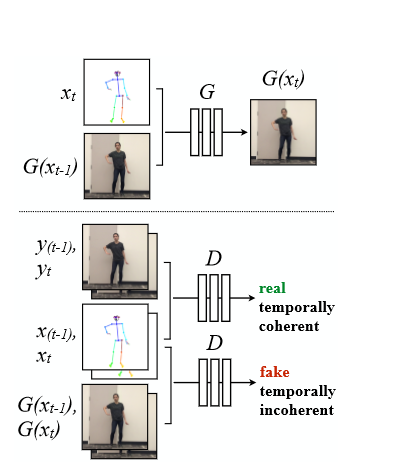
\includegraphics[scale=.5]{images/training2.png}
            \end{column}
            \begin{column}{0.5\textwidth}
                In order to create a smooth video, a temporal GAN setup is applied to slides with reference to their previous iterations.
                \vspace{0.2in}
                \begin{center}
                \end{center}
            \end{column}
        \end{columns}
    \end{frame}

\begin{frame}
        \frametitle{Objective}
        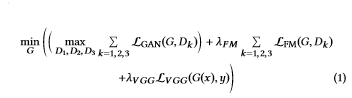
\includegraphics[scale=.6]{images/objective.png}\\
        \vspace{0.4in}
        face GAN objective is then applied\\
        \vspace{0.4in}
        \includegraphics[scale=.6]{images/faceGan.png}
    \end{frame}


\begin{frame}
        \frametitle{Results}
        The developed methods show improvement from the original pix2pixHD method. \\
        \begin{columns}
            \begin{column}{0.4\textwidth}
                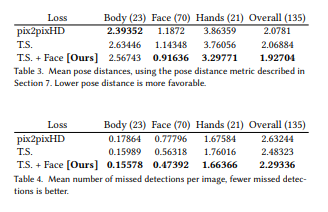
\includegraphics[scale=.8]{images/results2.png}
            \end{column}
            \begin{column}{0.6\textwidth}
                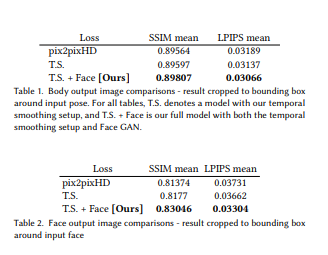
\includegraphics[scale=.8]{images/results1.png}
                \begin{center}
                \end{center}
            \end{column}
        \end{columns}
    \end{frame}

\end{document}